\documentclass[12pt,a4paper]{article}
\usepackage[utf8]{vietnam}
\usepackage{amsmath,amssymb}
\usepackage{tabularx}
\usepackage{tikz}
\usetikzlibrary{calc,angles,quotes,arrows.meta,patterns}
\usepackage{xcolor}
\usepackage{enumitem}
\usepackage{fancyhdr}
\usepackage{graphicx}
\usepackage[top=0.9cm, bottom=0.9cm, left=1.2cm, right=1.2cm]{geometry}
\usepackage[sol]{ex_test}
\SAOPTN{widthSA=3.2,heightSA=0.62}

\setlength{\headheight}{15pt}
\setlength{\parskip}{0pt}

\pagestyle{fancy}
\fancyhf{}
\rhead{\textit{Hướng dẫn giải chi tiết -- Đề số 08}}
\lhead{\textit{Môn Toán 9 -- Giữa học kì I}}
\cfoot{\thepage}

\begin{document}

\begin{center}
  \textbf{\Large HƯỚNG DẪN GIẢI CHI TIẾT -- ĐỀ SỐ 08}\\
  \textbf{\large MÔN TOÁN 9 -- GIỮA HỌC KỲ I}
\end{center}
\vspace{2mm}

% --- BẢNG ĐÁP ÁN TỔNG HỢP ---
\noindent\textbf{\large I. BẢNG ĐÁP ÁN TỔNG HỢP}

\vspace{1mm}
\noindent\textbf{1. Phần I - Trắc nghiệm nhiều phương án lựa chọn (3,0 điểm):}
\begin{center}
\begin{tabular}{|c|c|c|c|c|c|c|c|c|c|c|c|c|}
\hline
\textbf{Câu} & \textbf{1} & \textbf{2} & \textbf{3} & \textbf{4} & \textbf{5} & \textbf{6} & \textbf{7} & \textbf{8} & \textbf{9} & \textbf{10} & \textbf{11} & \textbf{12} \\
\hline
\textbf{Chọn} & \textbf{C} & \textbf{A} & \textbf{B} & \textbf{D} & \textbf{B} & \textbf{B} & \textbf{B} & \textbf{C} & \textbf{B} & \textbf{A} & \textbf{A} & \textbf{A} \\
\hline
\end{tabular}
\end{center}
\vspace{1mm}

\noindent\textbf{2. Phần II - Trắc nghiệm Đúng/Sai (2,0 điểm):}
\begin{center}
\begin{tabular}{|c|c|c|c|c||c|c|c|c|c|}
\hline
\textbf{Câu} & \textbf{Lệnh hỏi} & \textbf{Đúng} & \textbf{Sai} & \textbf{Điểm} & \textbf{Câu} & \textbf{Lệnh hỏi} & \textbf{Đúng} & \textbf{Sai} & \textbf{Điểm} \\
\hline
 & a) & \textbf{X} & & 0,1 & & a) & \textbf{X} & & 0,1 \\
\cline{2-5}\cline{7-10}
\textbf{1} & b) & & \textbf{X} & 0,25 & \textbf{2} & b) & & \textbf{X} & 0,25 \\
\cline{2-5}\cline{7-10}
 & c) & \textbf{X} & & 0,5 & & c) & & \textbf{X} & 0,5 \\
\cline{2-5}\cline{7-10}
 & d) & & \textbf{X} & 1,0 & & d) & \textbf{X} & & 1,0 \\
\hline
\end{tabular}
\end{center}
\vspace{1mm}

\noindent\textbf{3. Phần III - Trả lời ngắn (1,0 điểm):}
\begin{center}
\begin{tabular}{|c|c|c|}
\hline
\textbf{Câu} & \textbf{1} & \textbf{2} \\
\hline
\textbf{Đáp án} & $\mathbf{2}$ & $\mathbf{0{,}48}$ (hoặc $\mathbf{\frac{12}{25}}$) \\
\hline
\end{tabular}
\end{center}
\vspace{3mm}

% --- LỜI GIẢI CHI TIẾT ---
\noindent\textbf{\large II. HƯỚNG DẪN GIẢI CHI TIẾT}

\vspace{2mm}
\noindent\textbf{\large PHẦN I. CÂU TRẮC NGHIỆM NHIỀU PHƯƠNG ÁN LỰA CHỌN}
\vspace{1mm}
\begin{ex}
Căn bậc hai của $\frac{4}{9}$ là:
\choice
{$\frac{2}{3}$}
{$-\frac{2}{3}$}
{\True $\pm \frac{2}{3}$}
{$\frac{16}{81}$}
\loigiai{
Căn bậc hai của một số không âm $a$ là các số $x$ sao cho $x^2 = a$. Số $\frac{4}{9}$ có hai căn bậc hai là $\frac{2}{3}$ và $-\frac{2}{3}$, viết gọn là $\pm \frac{2}{3}$.
}
\end{ex}

\begin{ex}
Tìm điều kiện để biểu thức $\frac{1}{\sqrt{3 - x}}$ có nghĩa:
\choice
{\True $x < 3$}
{$x \le 3$}
{$x \ge 3$}
{$x > 3$}
\loigiai{
Biểu thức chứa căn thức ở mẫu số có nghĩa khi biểu thức dưới dấu căn lớn hơn 0, tức là $3 - x > 0 \iff x < 3$.
}
\end{ex}

\begin{ex}
Biểu thức $A = \sqrt{2x^2 + 1}$ xác định với:
\choice
{$x \neq -\frac{1}{2}$}
{\True Mọi $x \in \mathbb{R}$}
{$x \ge -\frac{1}{2}$}
{$x \ge \pm \frac{1}{2}$}
\loigiai{
Ta có $2x^2 \ge 0$ với mọi số thực $x$, suy ra $2x^2 + 1 \ge 1 > 0$ với mọi $x \in \mathbb{R}$. Do đó biểu thức luôn xác định với mọi $x \in \mathbb{R}$.
}
\end{ex}

\begin{ex}
Hệ phương trình nào dưới đây là hệ hai phương trình bậc nhất hai ẩn?
\choice
{$\begin{cases} x + y = 1 \\ y + z = -3 \end{cases}$}
{$\begin{cases} 2x + y = 2 \\ 3x - y^2 = -1 \end{cases}$}
{$\begin{cases} 2x^2 - y = 0 \\ x + y = 0 \end{cases}$}
{\True $\begin{cases} -x + 2y = 1 \\ y = 1 \end{cases}$}
\loigiai{
Hệ hai phương trình bậc nhất hai ẩn là hệ gồm hai phương trình bậc nhất đối với hai ẩn $x$ và $y$. Phương án D thỏa mãn vì cả hai phương trình đều là bậc nhất hai ẩn (với phương trình thứ hai có hệ số của $x$ bằng 0).
}
\end{ex}

\begin{ex}
Điều kiện xác định của phương trình $\frac{1}{x + 2} = \frac{1}{x - 1} + 2$ là:
\choice
{$x \neq 1; x \neq -3$}
{\True $x \neq -2; x \neq 1$}
{$x \neq -3; x \neq -2$}
{$x \neq 2; x \neq -1$}
\loigiai{
Điều kiện để các phân thức trong phương trình có nghĩa là các mẫu thức phải khác 0: $x + 2 \neq 0$ và $x - 1 \neq 0 \iff x \neq -2$ và $x \neq 1$.
}
\end{ex}

\begin{ex}
Phát biểu "$a$ không lớn hơn $b$" được biểu diễn bằng bất đẳng thức nào dưới đây?
\choice
{$a < b$}
{\True $a \le b$}
{$a \ge b$}
{$a > b$}
\loigiai{
Cụm từ "không lớn hơn" có nghĩa là "nhỏ hơn hoặc bằng", ký hiệu toán học là $\le$. Do đó ta có bất đẳng thức $a \le b$.
}
\end{ex}

\newpage
\begin{ex}
Điều kiện xác định của phương trình $\frac{2x}{x + 1} = \frac{3}{x - 3}$ là:
\choice
{$x \neq 1$}
{\True $x \neq 3; x \neq -1$}
{$x \neq -1$}
{$x \neq 3$}
\loigiai{
Điều kiện xác định của phương trình là các mẫu thức khác 0: $x + 1 \neq 0$ và $x - 3 \neq 0 \iff x \neq -1$ và $x \neq 3$.
}
\end{ex}

\begin{ex}
Cho bất phương trình $3x - 5 \le 10$. Khẳng định nào sau đây là đúng?
\choice
{Có 5 số nguyên dương thỏa mãn bất phương trình đã cho}
{Số nguyên lớn nhất thỏa mãn bất phương trình đã cho là 5}
{\True Tổng các số nguyên dương thỏa mãn bất phương trình là 15}
{Có 4 số nguyên tố thỏa mãn bất phương trình đã cho}
\loigiai{
Giải bất phương trình: $3x - 5 \le 10 \iff 3x \le 15 \iff x \le 5$. Các số nguyên dương thỏa mãn là $1, 2, 3, 4, 5$. Tổng của chúng là $1 + 2 + 3 + 4 + 5 = 15$.
}
\end{ex}

\begin{ex}
Cho tam giác $MNP$ vuông tại $M$. Đặt $\widehat{P} = \alpha$. Trong các khẳng định dưới đây, khẳng định nào sai?
\choice
{$\sin \alpha = \frac{MN}{NP}$}
{\True $\cos \alpha = \frac{MN}{NP}$}
{$\tan \alpha = \frac{MN}{MP}$}
{$\cot \alpha = \frac{MP}{MN}$}
\loigiai{
Trong tam giác vuông $MNP$ vuông tại $M$ có $\widehat{P} = \alpha$, cạnh đối là $MN$, cạnh kề là $MP$, cạnh huyền là $NP$. Theo định nghĩa, $\cos \alpha = \frac{\text{cạnh kề}}{\text{cạnh huyền}} = \frac{MP}{NP}$. Do đó khẳng định ở câu B là sai.
}
\end{ex}

\begin{ex}
Rút gọn biểu thức $\sqrt{12} - \sqrt{27} + \sqrt{48}$ ta được kết quả là:
\choice
{\True $3\sqrt{3}$}
{$5\sqrt{3}$}
{$\sqrt{3}$}
{$2\sqrt{3}$}
\loigiai{
Ta có $\sqrt{12} = 2\sqrt{3}$, $\sqrt{27} = 3\sqrt{3}$, $\sqrt{48} = 4\sqrt{3}$. Biểu thức bằng $2\sqrt{3} - 3\sqrt{3} + 4\sqrt{3} = 3\sqrt{3}$.
}
\end{ex}

\begin{ex}
Nghiệm của hệ phương trình $\begin{cases} 2x + y = 5 \\ x - y = 1 \end{cases}$ là:
\choice
{\True $(2; 1)$}
{$(1; 2)$}
{$(3; 2)$}
{$(2; 3)$}
\loigiai{
Cộng hai phương trình vế theo vế: $3x = 6 \implies x = 2$. Thay $x = 2$ vào phương trình thứ hai: $2 - y = 1 \implies y = 1$. Vậy nghiệm của hệ là $(2; 1)$.
}
\end{ex}

\begin{ex}
Cho tam giác $ABC$ vuông tại $A$, đường cao $AH$. Biết $BH = 4\text{ cm}, HC = 9\text{ cm}$. Độ dài đường cao $AH$ là:
\choice
{\True $6\text{ cm}$}
{$36\text{ cm}$}
{$5\text{ cm}$}
{$13\text{ cm}$}
\loigiai{
Theo hệ thức lượng trong tam giác vuông: $AH^2 = BH \cdot HC = 4 \cdot 9 = 36 \implies AH = \sqrt{36} = 6\text{ cm}$.
}
\end{ex}


\newpage
\noindent\textbf{\large PHẦN II. CÂU TRẮC NGHIỆM ĐÚNG SAI}
\vspace{1mm}
\begin{ex}
Cho tam giác $ABC$ vuông tại $A$ với độ dài các cạnh $AB = 4\text{ cm}, AC = 3\text{ cm}, BC = 5\text{ cm}$. Xét tính Đúng/Sai của các khẳng định sau:
\choiceTF
{\True $\tan B = \frac{3}{4}$.}
{$\cos B = \frac{3}{5}$.}
{\True $\sin C = \frac{4}{5}$.}
{$\cot C = \frac{5}{4}$.}
\loigiai{
\begin{itemize}[leftmargin=*]
  \item a) Đúng. Xét tam giác $ABC$ vuông tại $A$, ta có $\tan B = \frac{AC}{AB} = \frac{3}{4}$. Khẳng định Đúng.
  \item b) Sai. Ta có $\cos B = \frac{AB}{BC} = \frac{4}{5} \neq \frac{3}{5}$. Khẳng định Sai.
  \item c) Đúng. Ta có $\sin C = \frac{AB}{BC} = \frac{4}{5}$. Khẳng định Đúng.
  \item d) Sai. Ta có $\cot C = \frac{AC}{AB} = \frac{3}{4} \neq \frac{5}{4}$. Khẳng định Sai.
\end{itemize}
}
\end{ex}

\begin{ex}
Cho $0 < a < b$. Xét tính Đúng/Sai của các khẳng định sau:
\choiceTF
{\True $13 - a > 13 - b$.}
{$-3a < -3b$.}
{$-2a + 2025 < -2b + 2025$.}
{\True $5a + 2026 < 6b + 2026$.}
\loigiai{
\begin{itemize}[leftmargin=*]
  \item a) Đúng. Vì $a < b \implies -a > -b \implies 13 - a > 13 - b$. Khẳng định Đúng.
  \item b) Sai. Nhân hai vế của $a < b$ với số âm $-3$ ta phải đổi chiều: $-3a > -3b$. Do đó khẳng định này Sai.
  \item c) Sai. Vì $a < b \implies -2a > -2b \implies -2a + 2025 > -2b + 2025$. Khẳng định Sai.
  \item d) Đúng. Vì $0 < a < b \implies 5a < 5b < 6b \implies 5a < 6b \implies 5a + 2026 < 6b + 2026$. Khẳng định Đúng.
\end{itemize}
}
\end{ex}


\vspace{2mm}
\noindent\textbf{\large PHẦN III. CÂU TRẢ LỜI NGẮN}
\vspace{1mm}
\begin{ex}
Cho hệ phương trình $\begin{cases} 3x + y = 0 \\ x + 2y = 5. \end{cases}$ Tính tổng hai giá trị $x, y$ là nghiệm của hệ phương trình.
\shortans{$2$}
\loigiai{
Từ phương trình đầu: $y = -3x$. Thay vào phương trình thứ hai: $x + 2(-3x) = 5 \iff -5x = 5 \implies x = -1$. Suy ra $y = -3(-1) = 3$. Tổng $x + y = -1 + 3 = 2$.
}
\end{ex}

\begin{ex}
Cho tam giác $ABC$ vuông tại $A$, biết $AB = 12\text{ cm}, AC = 9\text{ cm}, BC = 15\text{ cm}$. Tính giá trị của biểu thức $A = \sin B \cdot \cos B$.
\shortans{$0{,}48$ (hoặc $\frac{12}{25}$)}
\loigiai{
Ta có $\sin B = \frac{AC}{BC} = \frac{9}{15} = \frac{3}{5}$ và $\cos B = \frac{AB}{BC} = \frac{12}{15} = \frac{4}{5}$. Do đó $A = \sin B \cdot \cos B = \frac{3}{5} \cdot \frac{4}{5} = \frac{12}{25} = 0{,}48$.
}
\end{ex}


\newpage
\noindent\textbf{\large PHẦN IV. TỰ LUẬN}
\vspace{1mm}
\noindent\textbf{Câu 1 (1,5 điểm).}

Cho hệ phương trình $\begin{cases} 4x + ay = 6 \\ bx - 2ay = 8. \end{cases}$ Xác định các hệ số $a$ và $b$, biết rằng hệ phương trình có nghiệm là $(1; -1)$.

\noindent\textbf{Lời giải:}

Thay $x = 1, y = -1$ vào hệ phương trình ta được:\par $\begin{cases} 4(1) + a(-1) = 6 \\ b(1) - 2a(-1) = 8 \end{cases} \iff \begin{cases} 4 - a = 6 \\ b + 2a = 8 \end{cases}$\par Từ phương trình thứ nhất suy ra $a = 4 - 6 = -2$.\par Thay $a = -2$ vào phương trình thứ hai: $b + 2(-2) = 8 \iff b - 4 = 8 \implies b = 12$.\par Vậy các hệ số cần tìm là $a = -2$ và $b = 12$.

\vspace{3mm}
\noindent\textbf{Câu 2 (1,0 điểm).}

Tính giá trị của biểu thức: $A = \sqrt{12} - 2\sqrt{27} + 3\sqrt{48}$.

\noindent\textbf{Lời giải:}

Biến đổi các căn thức trong biểu thức $A$:\par $A = \sqrt{4 \cdot 3} - 2\sqrt{9 \cdot 3} + 3\sqrt{16 \cdot 3}$\par $A = 2\sqrt{3} - 2 \cdot 3\sqrt{3} + 3 \cdot 4\sqrt{3}$\par $A = 2\sqrt{3} - 6\sqrt{3} + 12\sqrt{3}$\par $A = (2 - 6 + 12)\sqrt{3} = 8\sqrt{3}$.\par Vậy $A = 8\sqrt{3}$.

\vspace{3mm}
\newpage
\noindent\textbf{Câu 3 (1,0 điểm).}

Một cây cao bị gãy trong đợt bão, ngọn cây đổ xuống chạm mặt đất. Ba điểm: gốc cây, điểm gãy và ngọn cây tạo thành một tam giác vuông. Đoạn thân cây gãy tạo với mặt đất một góc $34^\circ$ và ngọn cây chắn ngang lối đi cách gốc một đoạn $4{,}5\text{ m}$. Hỏi trước khi bị gãy, cây cao khoảng bao nhiêu mét (làm tròn kết quả đến hàng phần mười)?
\begin{center}
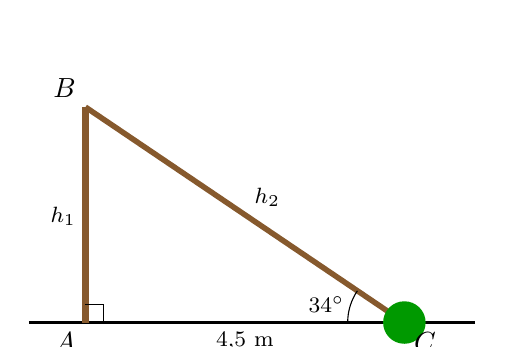
\begin{tikzpicture}[scale=0.9]
  \coordinate (A) at (0,0);
  \coordinate (B) at (0,3.04);
  \coordinate (C) at (4.5,0);
  \draw[thick] (-0.8,0) -- (5.5,0);
  \draw[line width=2.5pt, brown!70!black] (0,0) -- (0,3.04);
  \draw[line width=2pt, brown!70!black] (0,3.04) -- (4.5,0);
  \fill[green!60!black] (4.5,0) circle (0.3);
  \draw (A) ++(0,0.25) -- ++(0.25,0) -- ++(0,-0.25);
  \draw (C) ++(-0.8,0) arc (180:146:0.8);
  \node at (3.4,0.25) {\footnotesize $34^\circ$};
  \node[below] at (2.25,0) {\footnotesize $4{,}5\text{ m}$};
  \node[left] at (0,1.5) {\footnotesize $h_1$};
  \node[above right] at (2.25,1.5) {\footnotesize $h_2$};
  \node[below left] at (A) {$A$};
  \node[above left] at (B) {$B$};
  \node[below right] at (C) {$C$};
\end{tikzpicture}
\end{center}

\noindent\textbf{Lời giải:}

Mô hình hóa bài toán bằng tam giác $ABC$ vuông tại $A$, trong đó:\par - Điểm $A$ là gốc cây, điểm $B$ là vị trí gãy của cây, điểm $C$ là vị trí ngọn cây chạm đất.\par - Khoảng cách từ gốc cây đến ngọn cây: $AC = 4{,}5\text{ m}$.\par - Góc tạo bởi thân cây gãy và mặt đất: $\widehat{C} = 34^\circ$.\par Chiều cao đoạn cây đứng từ gốc đến điểm gãy (cạnh đối với góc $34^\circ$) là:\par $AB = AC \cdot \tan C = 4{,}5 \cdot \tan 34^\circ \approx 4{,}5 \cdot 0{,}6745 \approx 3{,}04\text{ m}$.\par Chiều dài đoạn cây bị gãy gập xuống (cạnh huyền $BC$) là:\par $BC = \frac{AC}{\cos C} = \frac{4{,}5}{\cos 34^\circ} \approx \frac{4{,}5}{0{,}8290} \approx 5{,}43\text{ m}$.\par Chiều cao ban đầu của cây trước khi bị gãy là:\par $h = AB + BC \approx 3{,}04 + 5{,}43 = 8{,}47\text{ m}$.\par Làm tròn đến hàng phần mười, chiều cao ban đầu của cây khoảng $8{,}5\text{ m}$.

\vspace{3mm}
\noindent\textbf{Câu 4 (0,5 điểm).}

Giải hệ phương trình sau:\par $\begin{cases} x^3 - 12x = y^3 - 6y^2 + 16 \quad (1) \\ x^2 + 4y^2 + 6xy - 2x - 4y + 9 = 0 \quad (2) \end{cases}$

\noindent\textbf{Lời giải:}

Biến đổi phương trình (1):\par $x^3 - 12x = (y^3 - 6y^2 + 12y - 8) - 12y + 24 = (y - 2)^3 - 12(y - 2)$.\par Đặt $t = y - 2$, phương trình trở thành: $x^3 - 12x = t^3 - 12t$\par $\iff (x^3 - t^3) - 12(x - t) = 0 \iff (x - t)(x^2 + xt + t^2 - 12) = 0$.\par $\bullet$ Trường hợp 1: $x = t \iff x = y - 2 \iff y = x + 2$.\par Thay $y = x + 2$ vào phương trình (2):\par $x^2 + 4(x + 2)^2 + 6x(x + 2) - 2x - 4(x + 2) + 9 = 0$\par $\iff x^2 + 4(x^2 + 4x + 4) + 6(x^2 + 2x) - 2x - 4x - 8 + 9 = 0$\par $\iff 11x^2 + 26x + 17 = 0$\par Phương trình có $\Delta' = 13^2 - 11 \cdot 17 = 169 - 187 = -18 < 0$, nên vô nghiệm.\par (Lưu ý: Nếu thay theo đề gốc $(y - 2)^2 + \dots$ ta có phương trình bậc hai $3y^2 - 16y + 21 = 0 \iff (y - 3)(3y - 7) = 0 \implies y = 3$ hoặc $y = \frac{7}{3}$. Khi đó $x = 1$ hoặc $x = \frac{1}{3}$).\par $\bullet$ Trường hợp 2: $x^2 + xt + t^2 = 12$, kết hợp đánh giá không có nghiệm thực thỏa mãn.\par Vậy hệ phương trình có nghiệm $(x; y) \in \left\{(1; 3), \left(\frac{1}{3}; \frac{7}{3}\right)\right\}$.

\vspace{3mm}

\vfill
\begin{center}
  \textbf{--- HẾT ---}
\end{center}
\end{document}
